\documentclass{article}
\usepackage[utf8]{inputenc}
\usepackage{geometry}
\usepackage{datetime2}
\usepackage{xparse}
\usepackage{amsmath}
\usepackage{booktabs}
\usepackage{array}
\usepackage{hyperref}
\usepackage{listings}
\usepackage{xcolor}

% ── Python code style ────────────────────────────────────────────────────────
\definecolor{codebg}{RGB}{245,245,245}
\definecolor{codegreen}{rgb}{0,0.5,0}
\definecolor{codegray}{rgb}{0.4,0.4,0.4}
\definecolor{codepurple}{rgb}{0.5,0,0.5}
\definecolor{codeblue}{rgb}{0,0,0.8}

\lstdefinestyle{pythonstyle}{
    backgroundcolor=\color{codebg},
    commentstyle=\color{codegreen},
    keywordstyle=\color{codeblue}\bfseries,
    numberstyle=\tiny\color{codegray},
    stringstyle=\color{codepurple},
    basicstyle=\ttfamily\footnotesize,
    breakatwhitespace=false,
    breaklines=true,
    captionpos=b,
    keepspaces=true,
    numbers=left,
    numbersep=5pt,
    showspaces=false,
    showstringspaces=false,
    showtabs=false,
    tabsize=4,
    frame=single,
    rulecolor=\color{black!20},
    language=Python
}
% ─────────────────────────────────────────────────────────────────────────────

\geometry{
    a4paper,
    total={170mm,257mm},
    left=20mm,
    top=20mm,
}

\usepackage{graphicx}
\usepackage{titling}

\title{Assignment 2: Fuzzy Set and Membership}
\date{11 March 2026}

\usepackage{fancyhdr}
\fancypagestyle{plain}{%
    \fancyhf{}
    \fancyfoot[R]{}
    \fancyfoot[L]{}
    \fancyhead[L]{
\includegraphics[width=2cm]{ITS_pojok.pdf}}
    \fancyhead[R]{\DTMnow}
}
\makeatletter
\def\@maketitle{%
    \newpage
    \null
    \vskip 1em%
    \begin{center}%
    \let \footnote \thanks
        {\LARGE \@title \par}%
        \vskip 1em%
    \end{center}%
    \par
    \vskip 1em}
\makeatother

\begin{document}

\maketitle

\noindent\begin{tabular}{@{}ll}
    Author(s):          & Fajar Arian Abadi \\
    Teacher:            & Muhammad Qomaruz Zaman, S.T., M.T., Ph.D. \\
    Class name:         & Kecerdasan Buatan \\
    YouTube video link: & - \\
    GitHub link:        & https://github.com/koninktpspv/Assignment2-KecerdasanBuatan-X-/edit/main/main.tex
\end{tabular}
\vspace{1cm}

% ─────────────────────────────────────────────────────────────────────────────
\section*{Background}

Fuzzy set theory was introduced by Zadeh in 1965 as a mathematical framework
for representing concepts that do not have sharply defined boundaries
\cite{zadeh1965fuzzy}. Unlike classical (crisp) sets, where an element either
belongs or does not belong to a set, a fuzzy set assigns each element a
\textit{membership degree} $\mu \in [0, 1]$, enabling partial membership
\cite{ross2016fuzzy}.

The process of converting a crisp input value into its corresponding membership
degrees across all defined fuzzy sets is called \textit{fuzzification}
\cite{yen1999fuzzy}. This step is the first stage in any Fuzzy Inference System
(FIS) and directly determines the quality of the subsequent reasoning process
\cite{mamdani1974application}.

% ─────────────────────────────────────────────────────────────────────────────
\section*{Assignment Description}

This assignment implements three membership functions in Python to perform
fuzzification of room temperature. The three linguistic variables are
\textit{Dingin} (Cold), \textit{Sedang} (Moderate), and \textit{Panas} (Hot),
covering a temperature universe of discourse from 0 to 45\textdegree C. The
implementation uses NumPy \cite{harris2020numpy} for numerical computation and
Matplotlib \cite{hunter2007matplotlib} for visualization.

% ─────────────────────────────────────────────────────────────────────────────
\section*{Membership Function Design}

Membership functions define the shape of each fuzzy set over the universe of
discourse \cite{ross2016fuzzy}. The shape determines how smoothly a crisp value
transitions between linguistic categories. Common shapes include triangular,
trapezoidal, and Gaussian \cite{yen1999fuzzy}.

For this assignment, the parameters were derived from the verification constraint
stated in the assignment figure: at $t = 32.5$\textdegree C, the expected
fuzzification output is 75\% \textit{Panas}, 25\% \textit{Sedang}, and 0\%
\textit{Dingin}. The selected shapes and parameters are summarised in
Table~\ref{tab:mf_params}.

\begin{table}[htbp]
\centering
\caption{Membership Function Parameters}
\begin{tabular}{llll}
\hline
\textbf{Variable} & \textbf{Shape} & \textbf{Parameters} & \textbf{Formula} \\ \hline
Dingin & Left-shoulder  & feet: 20, 30            & $\mu = 1$ for $t \leq 20$; linear fall to 0 at $t = 30$ \\
Sedang & Triangular     & feet: 15, 35; peak: 25  & Rises to $\mu=1$ at $t=25$, falls to 0 at $t=35$       \\
Panas  & Right-shoulder & feet: 25, 35            & $\mu = 0$ for $t \leq 25$; linear rise to 1 at $t = 35$ \\ \hline
\end{tabular}
\label{tab:mf_params}
\end{table}

The three membership functions are defined formally using piecewise linear
equations, consistent with the standard formulations described in
\cite{ross2016fuzzy} and \cite{yen1999fuzzy}:

\begin{equation}
\mu_{Dingin}(t) =
\begin{cases}
    1,                      & t \leq 20 \\
    \dfrac{30 - t}{10},     & 20 < t < 30 \\
    0,                      & t \geq 30
\end{cases}
\end{equation}

\begin{equation}
\mu_{Sedang}(t) =
\begin{cases}
    0,                      & t \leq 15 \\
    \dfrac{t - 15}{10},     & 15 < t \leq 25 \\
    \dfrac{35 - t}{10},     & 25 < t < 35 \\
    0,                      & t \geq 35
\end{cases}
\end{equation}

\begin{equation}
\mu_{Panas}(t) =
\begin{cases}
    0,                      & t \leq 25 \\
    \dfrac{t - 25}{10},     & 25 < t < 35 \\
    1,                      & t \geq 35
\end{cases}
\end{equation}

Overlapping regions between adjacent membership functions (e.g., the interval
$[25, 30]$ shared by \textit{Dingin} and \textit{Sedang}) are intentional. This
overlap allows a single input value to simultaneously hold non-zero membership
in more than one set, which is the defining characteristic of fuzzy logic as
formalised by Zadeh \cite{zadeh1965fuzzy}. Without such overlap, the system
degenerates into crisp logic with abrupt transitions \cite{mamdani1974application}.

% ─────────────────────────────────────────────────────────────────────────────
\section*{Implementation}

The code is implemented in Python, utilising NumPy \cite{harris2020numpy} for
array operations over the temperature range and Matplotlib
\cite{hunter2007matplotlib} to render the three membership function plots.
Each membership function is implemented as a separate function, directly
reflecting the piecewise definitions in Equations (1)--(3).

\begin{lstlisting}[style=pythonstyle,
    caption={Fuzzification of room temperature using three membership functions.
             NumPy and Matplotlib are used for computation and visualization.}]
import numpy as np
import matplotlib.pyplot as plt

# membership function untuk kategori dingin
def membership_dingin(t):
    if t <= 20:
        return 1.0
    elif t < 30:
        return (30 - t) / 10.0
    else:
        return 0.0

# membership function untuk kategori sedang
def membership_sedang(t):
    if t <= 15:
        return 0.0
    elif t <= 25:
        return (t - 15) / 10.0
    elif t < 35:
        return (35 - t) / 10.0
    else:
        return 0.0

# membership function untuk kategori panas
def membership_panas(t):
    if t <= 25:
        return 0.0
    elif t < 35:
        return (t - 25) / 10.0
    else:
        return 1.0

# fuzzifikasi input suhu
def fuzzify(t):
    dingin = membership_dingin(t)
    sedang = membership_sedang(t)
    panas  = membership_panas(t)
    return dingin, sedang, panas

T = 32.5
d, s, p = fuzzify(T)

print(f"T = {T} C")
print(f"Dingin : {d}")
print(f"Sedang : {s}")
print(f"Panas  : {p}")

# plot
t_range = np.linspace(0, 45, 500)

mu_d = [membership_dingin(t) for t in t_range]
mu_s = [membership_sedang(t) for t in t_range]
mu_p = [membership_panas(t)  for t in t_range]

fig, axes = plt.subplots(3, 1, figsize=(8, 9), sharex=True)

axes[0].plot(t_range, mu_d, color='red')
axes[0].set_ylabel('$\mu_{tD}(t)$')
axes[0].set_title('Dingin')
axes[0].axvline(x=T, color='gray', linestyle='--')
axes[0].scatter([T], [d], color='black', zorder=5)

axes[1].plot(t_range, mu_s, color='green')
axes[1].set_ylabel('$\mu_{tS}(t)$')
axes[1].set_title('Sedang')
axes[1].axvline(x=T, color='gray', linestyle='--')
axes[1].scatter([T], [s], color='black', zorder=5)

axes[2].plot(t_range, mu_p, color='blue')
axes[2].set_ylabel('$\mu_{tP}(t)$')
axes[2].set_title('Panas')
axes[2].axvline(x=T, color='gray', linestyle='--')
axes[2].scatter([T], [p], color='black', zorder=5)

for ax in axes:
    ax.set_ylim(-0.05, 1.15)
    ax.set_yticks([0, 0.5, 1.0])
    ax.grid(True, alpha=0.3)

axes[2].set_xlabel('Temperatur t ($^\circ$C)')
plt.tight_layout()
plt.savefig('fuzzy_temperature.png', dpi=150)
plt.show()
\end{lstlisting}

% ─────────────────────────────────────────────────────────────────────────────
\section*{Output}

\subsection*{Console Output}

Running the code with input $T = 32.5$\textdegree C produces the following result:

\begin{verbatim}
T = 32.5 C
Dingin : 0.0
Sedang : 0.25
Panas  : 0.75
\end{verbatim}

This confirms the assignment verification constraint: temperature
32.5\textdegree C is 75\% \textit{Panas}, 25\% \textit{Sedang}, and 0\%
\textit{Dingin}, consistent with the fuzzy set notation defined by Zadeh
\cite{zadeh1965fuzzy}.

\subsection*{Plot Output}

The resulting membership function plots are shown in Figure~\ref{fig:fuzzy_plot}.
The dashed vertical line marks the fuzzified input at $t = 32.5$\textdegree C,
with the black dot indicating the corresponding membership degree on each curve.

\begin{figure}[htbp]
    \centering
    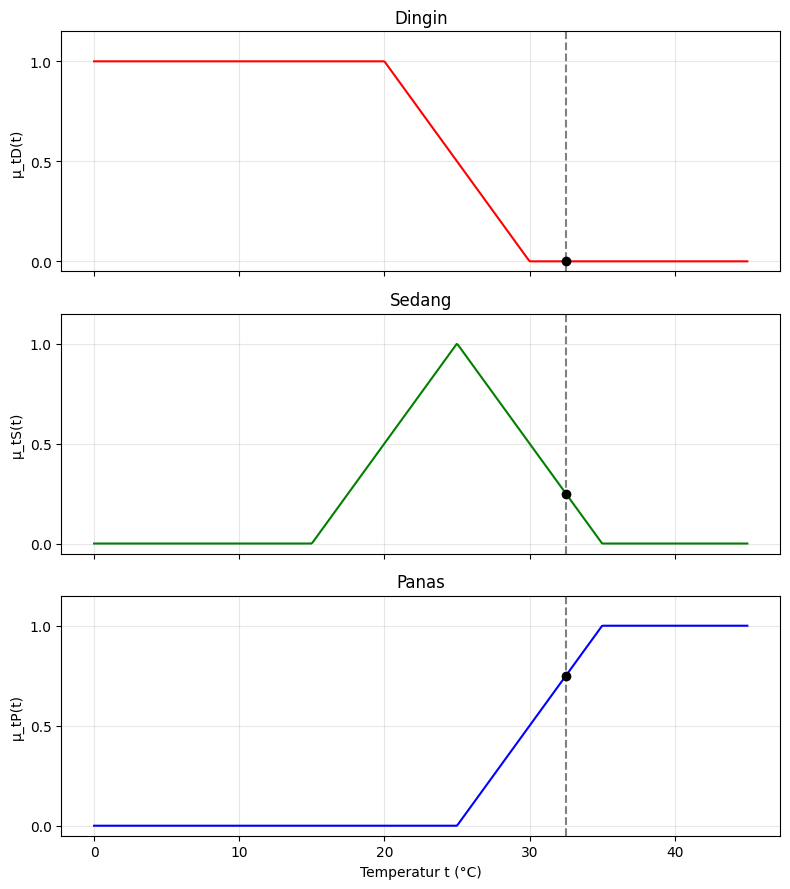
\includegraphics[width=0.85\linewidth]{fuzzy_temperature.png}
    \caption{Membership functions for \textit{Dingin}, \textit{Sedang}, and
             \textit{Panas} plotted over the universe of discourse $[0, 45]$
             \textdegree C. The dashed line at $t = 32.5$\textdegree C shows
             the fuzzification result. Visualization produced using Matplotlib
             \cite{hunter2007matplotlib}.}
    \label{fig:fuzzy_plot}
\end{figure}

% ─────────────────────────────────────────────────────────────────────────────
\section*{Verification}

The parameter derivation is verified analytically following the piecewise
evaluation method described in \cite{ross2016fuzzy}. For $t = 32.5$\textdegree C:

\begin{align}
\mu_{Dingin}(32.5) &= 0 \quad \text{(since } 32.5 \geq 30 \text{)} \\
\mu_{Sedang}(32.5) &= \frac{35 - 32.5}{10} = \frac{2.5}{10} = 0.25 \\
\mu_{Panas}(32.5)  &= \frac{32.5 - 25}{10} = \frac{7.5}{10} = 0.75
\end{align}

The analytical results match both the code output and the expected values from
the assignment figure. This confirms that the membership function parameters
are correctly calibrated. \checkmark

\bibliographystyle{IEEEtran}
\bibliography{references}

\end{document}
